\chapter[Use of the LTL Checker Plugins]{How to use the LTL Checker Plugins}
\label{plugingui}

\section{Introduction}
\label{plugingui:introduction}

This chapter is about how to use the LTL Checker plugins. There are three
different plugins which are all grouped under the name "LTL Checker plugins". These
plugins are an LTL Template Import plugin, a Default LTL Checker plugin and
the "normal" LTL Checker plugin.

\begin{figure}[H]
    \includegraphics[scale=0.3]{images/framework-start.eps}
    \caption{The ProM window after a first start.}
    \label{plugingui:start}
\end{figure}

The LTL Template Import plugin is a plugin to import LTL
Template files. LTL Template files are files containing the specification of properties written in
the special LTL Language ( Chapter \ref{language} ). After importing such files, the
properties specified in it can be used to check workflow logs of processes:
which instances of the processes have the property?

The actual check is performed by one of the LTL Checker plugins. The Default
LTL Checker plugin uses a standard LTL Template file with some common ltl
properties defined in it. By the "normal"  LTL Checker plugin there is no standard LTL
Template file, you can choose which LTL Template file you want to
use, just import that one.

Both the Default and the "normal" LTL Checker plugins are analysis plugins. These analysis plugins can
be used on all mined logs given an appropriate input. This means that if you
will use the LTL Checker plugin, you should first mine a log. Fortunately
there is an \textit{empty mining} plugin in the framework, using that "mining
algorithm" mining is reduced to just reading the log.

In the next sections of this chapter, all steps taken and windows encountered while
using one of the LTL Checker plugins are explained in full detail. The first
plugin to be explained is the LTL Template Import plugin.

\section{Importing LTL Template Files}
\label{plugingui:importing}
\index{LTL Template Import Plugin!How to use}
\index{Importing LTL Template files}
\index{Importing in the ProM framework!LTL Template files}

The window of the ProM framework will look like the window displayed in Figure
\ref{plugingui:start}. In this figure the window of ProM is displayed directly
after starting ProM. While using ProM, thus after mining,
importing and analyzing, this window may be filled with many internal windows.
Because the goal of this chapter is to teach you how
to use the LTL Checker plugins, it is assumed that you start ProM from scratch, just to
keep things simple.

\begin{figure}[H]
    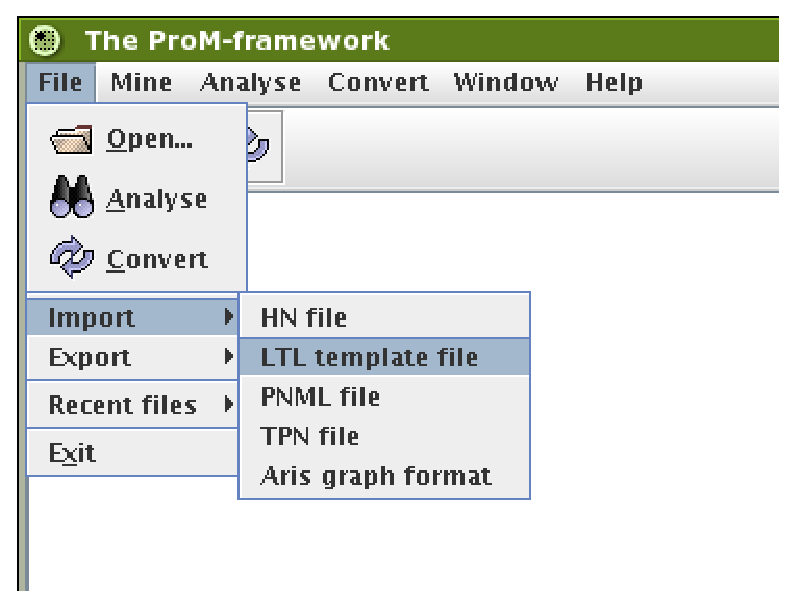
\includegraphics[scale=0.5]{images/framework-import-menu-cutted.eps}
    \caption{The import menu.}
    \label{plugingui:importmenu}
\end{figure}

For importing an LTL Template File, you go to the \menu{File}-menu, and then to
the sub menu \menu{Import}. In this menu you can choose one of the items
listed ( Figure \ref{plugingui:importmenu} ), one of items is \menu{LTL template file}. Click on
this item and a new open dialog is displayed.

\begin{figure}[H]
    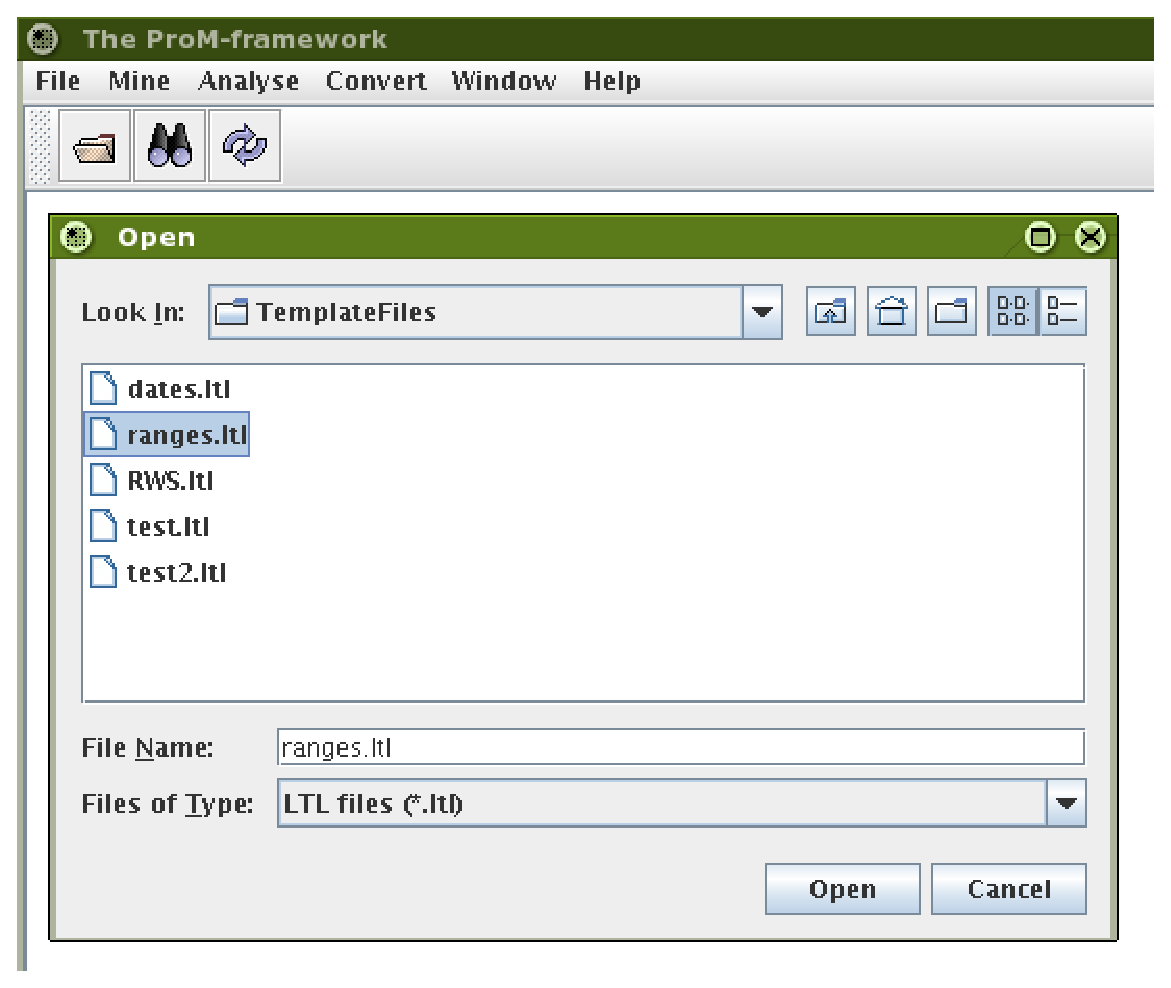
\includegraphics[scale=0.5]{images/framework-import-opendialog.eps}
    \caption{The open dialog for importing LTL Template files.}
    \label{plugingui:opendialog}
\end{figure}

In this dialog, you navigate to the directory containing the LTL Template file
you want to import, select this file, and click the \menu{Open} button ( Figure
\ref{plugingui:opendialog} ). It is a good custom to
give your LTL Template files the extension \textbf{.ltl} because you
will more easily recognize your ltl-files, and in the open dialog files are
initially filtered on this extension.

\begin{figure}[H]
    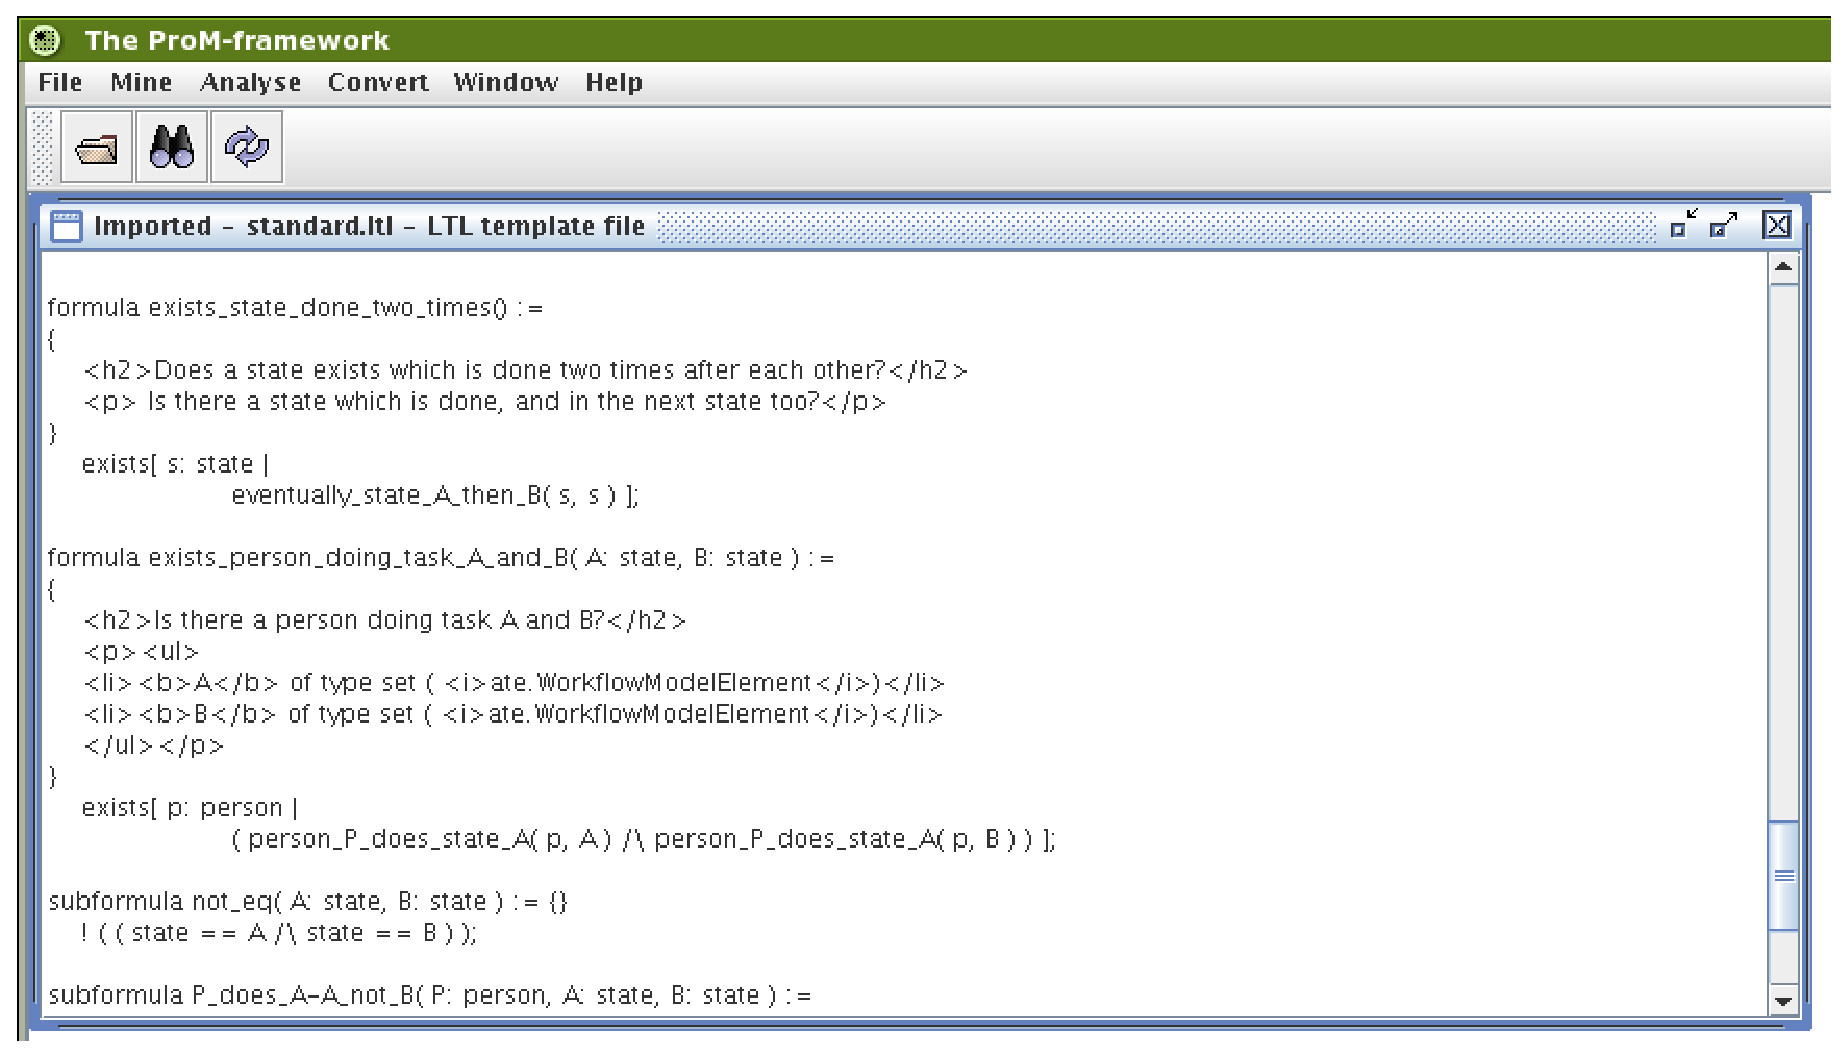
\includegraphics[scale=0.4]{images/framework-import-opened-cutted.eps}
    \caption{The contents of the imported LTL Template file are displayed.}
    \label{plugingui:openwindow}
\end{figure}

Now the framework tries to open the LTL Template file. The file is parsed by the LTL Parser and the
contents of the file are putted in a \textit{read-only} text box. This
window, you see it on Figure \ref{plugingui:openwindow}, has no functionality
at all, but may be, in some future it will become more elaborate. 

Now the import has succeeded, as you can see in the message pane at the bottom
of the ProM framework window:
\texttt{Parsing complete. /home/\-htdebeer/\-TestLTL/\-test11.ltl imported.}
Of course you will see the path and filename of your imported file, but the
message is clear.

If the import does not result in success, a message is also given in the
message pane: \texttt{Importing of /home/\-htdebeer/\-TestLTL/\-test01.ltl aborted.}
In the message pane under the tab \textit{error} can you find the error
message, which gives the reason why or a hint how to solve the problem. For
more information about the parse error messages, have a look in the next
chapter.

\section{Using the stand alone LTL Parser}
\label{plugingui:parser}
\index{LTL Parser!Use on the command line}

Happily the LTL Parser is also available as a stand alone program, so
for debugging your own LTL Template files, you do not need to start ProM. The
stand alone LTL Parser can be started by typing the following on the command
line, assuming you are in the base directory of ProM:\\

\texttt{java -classpath "lib/plugins/ltlchecker.jar" $\hookleftarrow$\\
org.processmining.analysis.ltlchecker.parser.LTLParser $\hookleftarrow$\\
\textit{file\_to\_parse}}. When you are using the DOS operating system, you
have to change the slashes into backslashes. The LTL Parser expects exactly
one filename.

If the parsing is successful, no message is send to standard out, the prompt
returns directly. If there is an error while parsing, a message is send to standard
out, consisting of the kind of error, and on the next line the message of
the error. There are three kinds of errors possible:
\index{LTL Parser!Error messages}
\begin{enumerate}
    \item \texttt{Error occurred during parsing:} The file is opened, but the
    contents are not parseble by the LTL Parser. The most likely reason is
    that you have made an error by writing ltl expressions.
    \item \texttt{Error while reading \textit{filename}. Check the file(name)
    and try again.} There are problems with opening and reading the file.
    Maybe the file does not exist or it is already in use by another program.
    \item \texttt{Unknown error:} All errors not of kind one or two are
    unknown, that is, they are not expected by the parser but are thrown
    nonetheless. Most likely it is then a bug, so send a bug report containing
    the error message, and LTL Template file you try to import.
\end{enumerate}

\section{Starting the Default LTL Checker Plugin}
\label{plugingui:default}
\index{LTL Checker Plugin!Default!How to start}

\begin{figure}[H]
    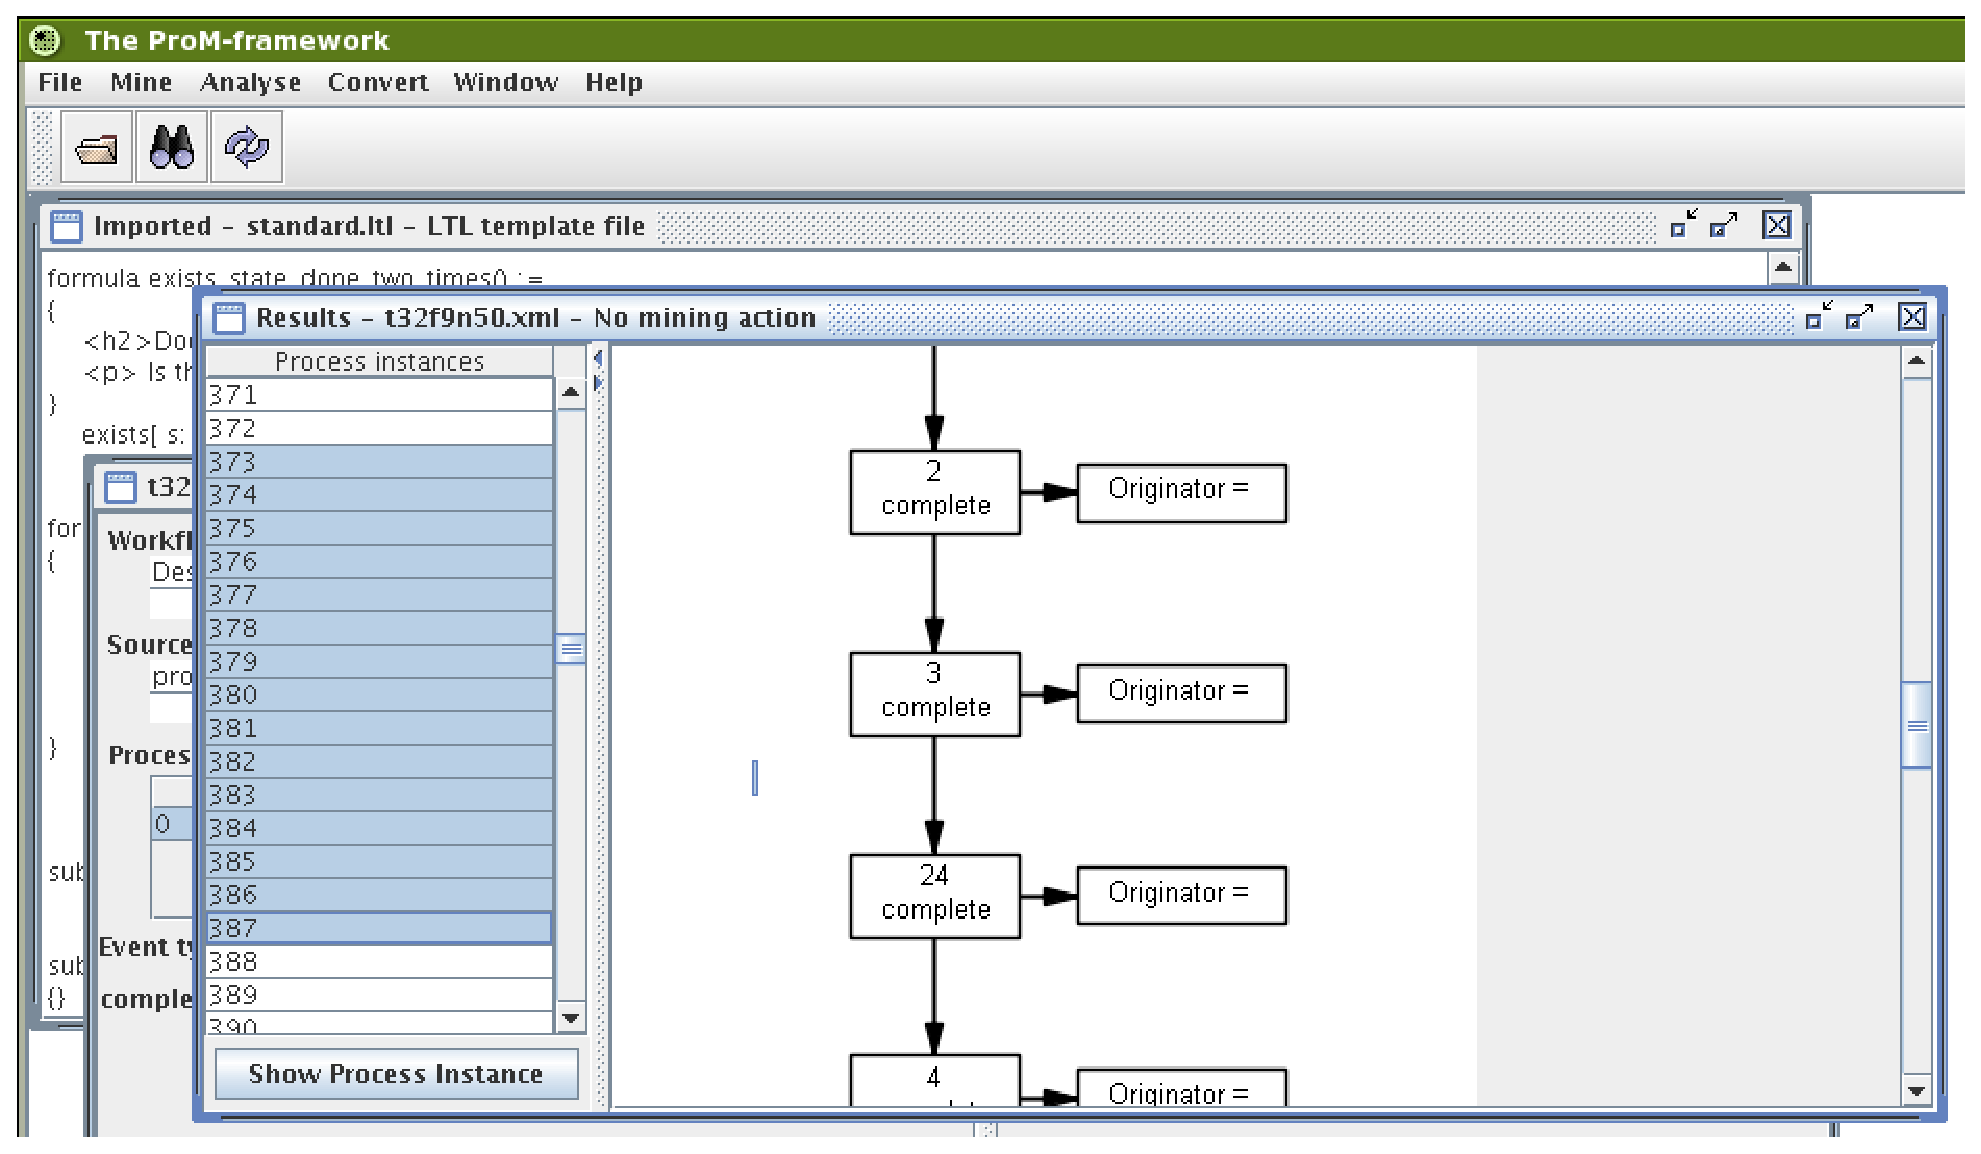
\includegraphics[scale=0.4]{images/framework-log-and-ltl-cutted.eps}
    \caption{A log is mined with the \textit{No mining action} mining plugin.}
    \label{plugingui:log}
\end{figure}

How to start the Default LTL Checker plugin is explained in this section. The Default LTL Checker Plugin can be started on \textit{every} (mined)
log, that is, the active internal window of the ProM framework window should
contain such log. For now, we open just a log an mine it with the \menu{No
mining action} mining algorithm ( Figure \ref{plugingui:log} ). This mining
plugin does nothing but read the log and displays the contents of it in a new
window. If you want, you can visualize one process instance.

\begin{figure}[H]
    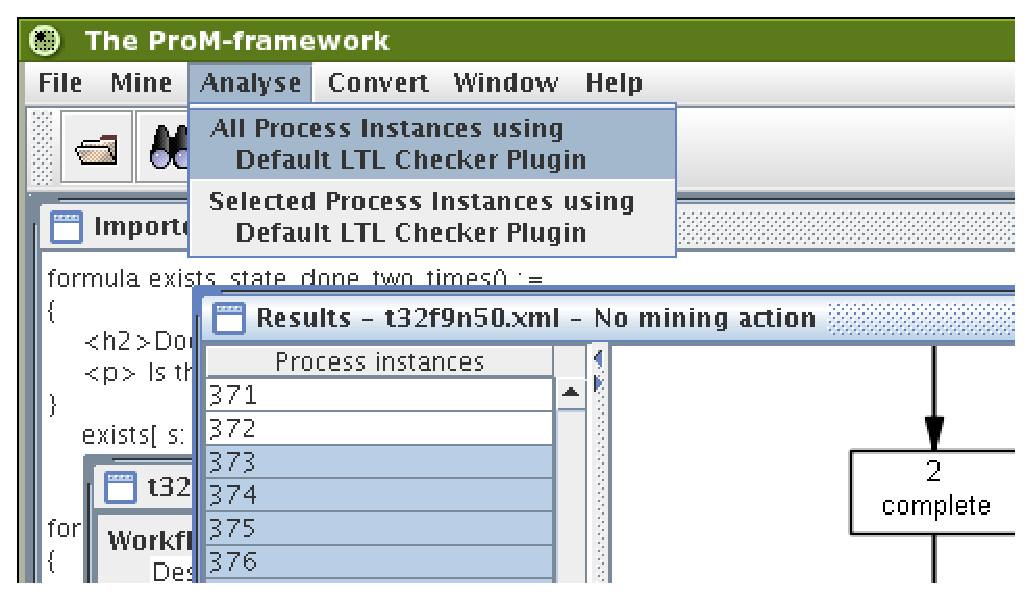
\includegraphics[scale=0.5]{images/framework-log-and-ltl-defaultmenu-cutted.eps}
    \caption{The analyze menu to start the Default LTL Checker Plugin.}
    \label{plugingui:analysemenu}
\end{figure}

Now, with this new window ( or another log) activated so that it is the only
active internal window of the ProM framework window, you can run the Default
LTL Checker plugin via the menu \menu{Analyze}, as is displayed in figure
\ref{plugingui:analysemenu}. After clicking one of the Default LTL Checker
Plugin menu items, a new window is opened: the Template GUI ( Section
\ref{plugingui:templategui} ).

The Default LTL Checker plugin can also be started as you can the LTL
Checker plugin, but that is explained later.

Internally the standard LTL Template file\index{Standard LTL Template file} is
parsed. This file, called \texttt{standard.ltl} and can be found in the
lib/plugins subdirectory of the ProM base directory. You can change the
contents of this file to your own needs. But, here again, it is a good idea to
try to parse a new standard ltl file before you use it ( Section
\ref{plugingui:parser} ). If the standard file can not be opened or parsed, a message box is shown with
the error message in it.

\section{Starting The LTL Checker Plugin}
\label{plugingui:checker}
\index{LTL Checker Plugin!LTL Checker Plugin!How to start}

While the Default LTL Checker Plugin does not need an imported LTL Template
file, the LTL Checker Plugin must have access to at least one such
imported file. Here too, as was the case for the default plugin, you should
have an opened ( and mined) log to use this plugin.

Once you have both, log and LTL Template file, you can start the LTL
Checker Plugin by opening the \menu{Analysis} window. This plugin can
not be accessed through the \menu{Analyses} menu because it needs two inputs:
a log and an LTL Template file, it is up to you to select the appropriate input.

\begin{figure}[H]
    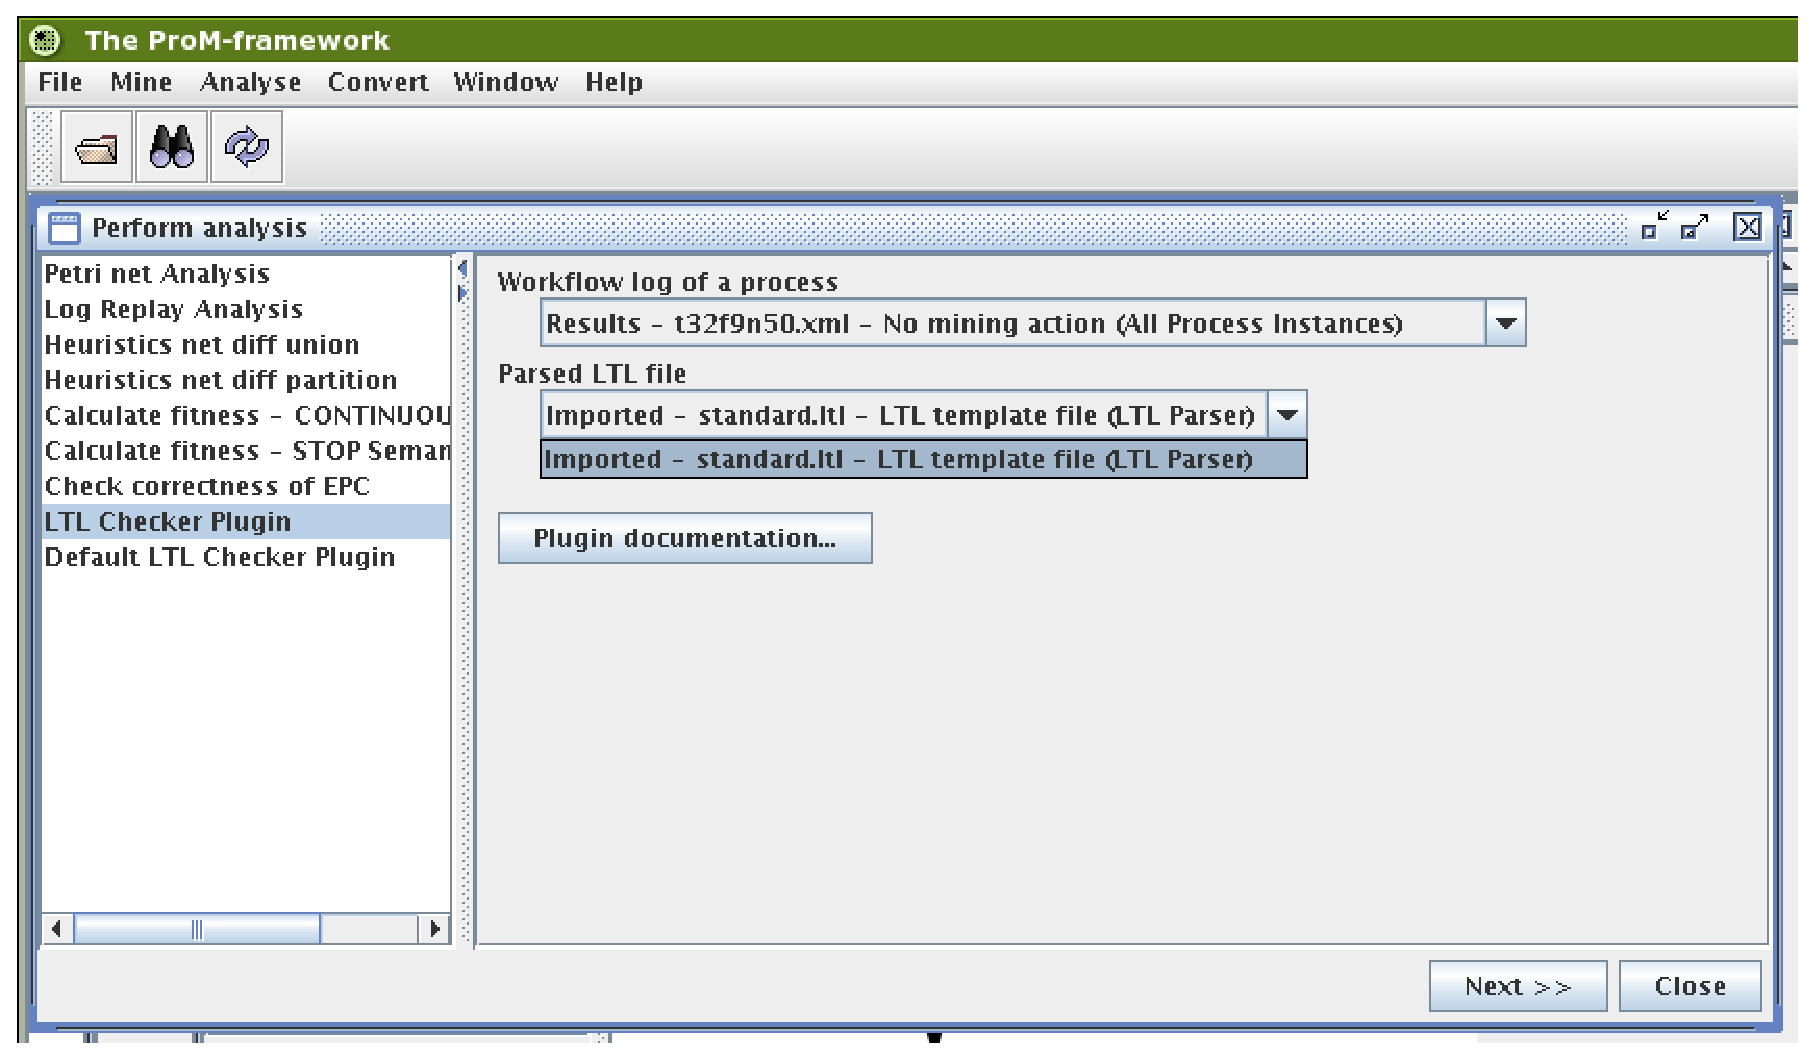
\includegraphics[scale=0.4]{images/framework-log-and-ltl-analyse-cutted.eps}
    \caption{The analyze window.}
    \label{plugingui:analysewindow}
\end{figure}

You can open the Analyze window by clicking on the \textit{binoculars} button
on the toolbar ( or press \texttt{ALT + A}). This window is displayed in
Figure \ref{plugingui:analysewindow}. As you can see, on the left hand side of
the window you can select an analyze plugin. In this case you will select the
LTL Checker Plugin. But as said before you can also select the Default LTL
Checker plugin.

On the right hand side of the window you can select the log to check (the
first combo box) and the imported LTL Template file in which the property to
check can be found. Now the LTL Checker Plugin has enough information to start, so
click the \menu{Next} button and a new internal window is displayed: the Template GUI.

\section{Using the Template GUI}
\label{plugingui:templategui}
\index{LTL Checker Plugin!How to use the Template GUI}
\index{Template GUI}

\begin{figure}[H]
    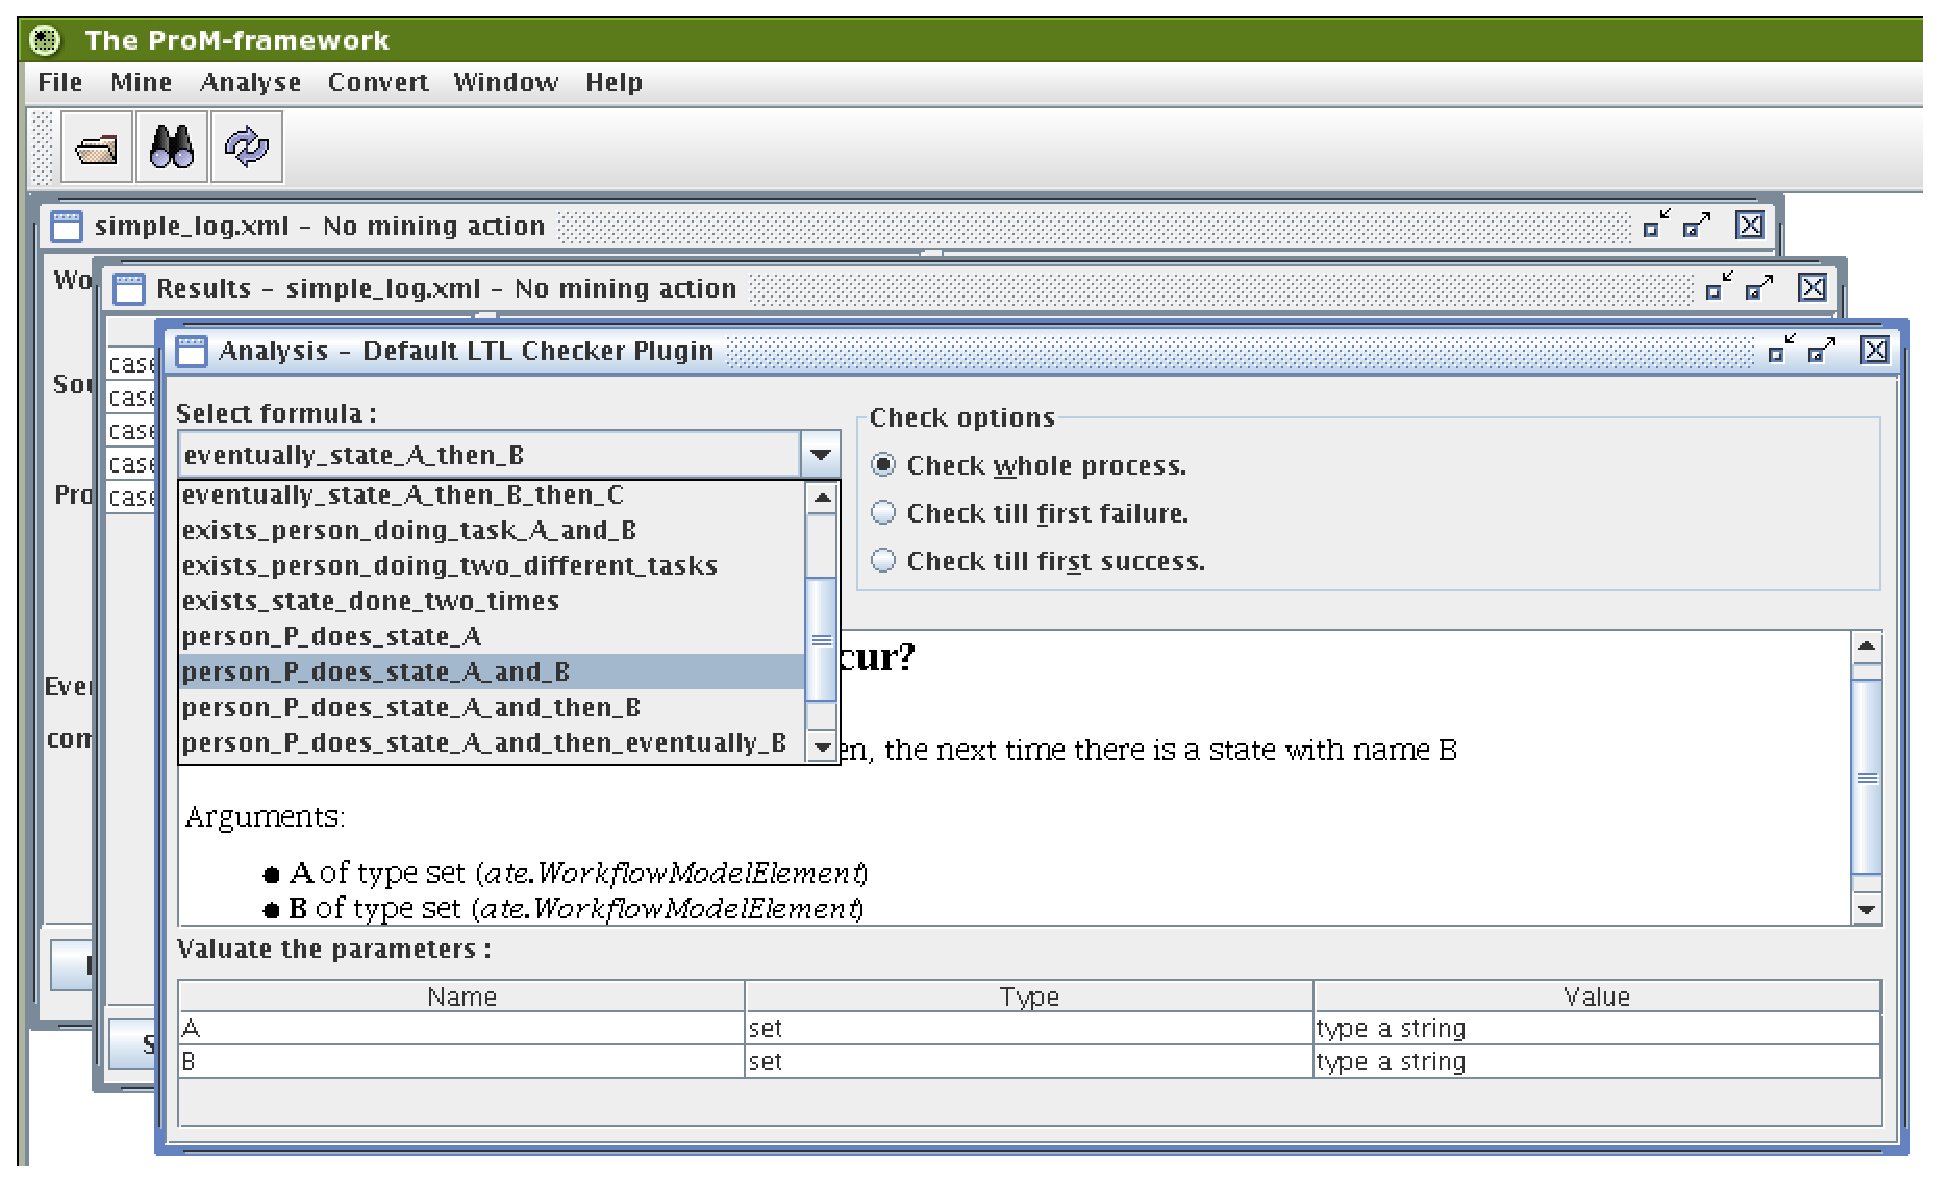
\includegraphics[scale=0.4]{images/ltlchecker-choose-formula-cutted.eps}
    \caption{Choosing a formula in the Template GUI.}
    \label{plugingui:chooseformula}
\end{figure}

The Template GUI is a window consisting of four parts and a check button. The
first part is a list of formula names from which you can choose a formula.
This selected formula is used to check on the log. 

Initially the first formula of the list is selected. If no formulae are
defined the item \textit{no formulae} is visible and selected. In the second
part of the window, the description pane, you will see the description, if
any, of the selected formula ( Figure \ref{plugingui:chooseformula} ).
If the imported LTL Template file is created with care, there should be a
description for every formula. If not, just guess what the meaning is of the
selected formula. 

The third part of the window is the parameter table. If the selected formula
has any parameters these parameters are shown in this parameter table ( Figure
\ref{plugingui:valuateparameters} ).

\begin{figure}[H]
    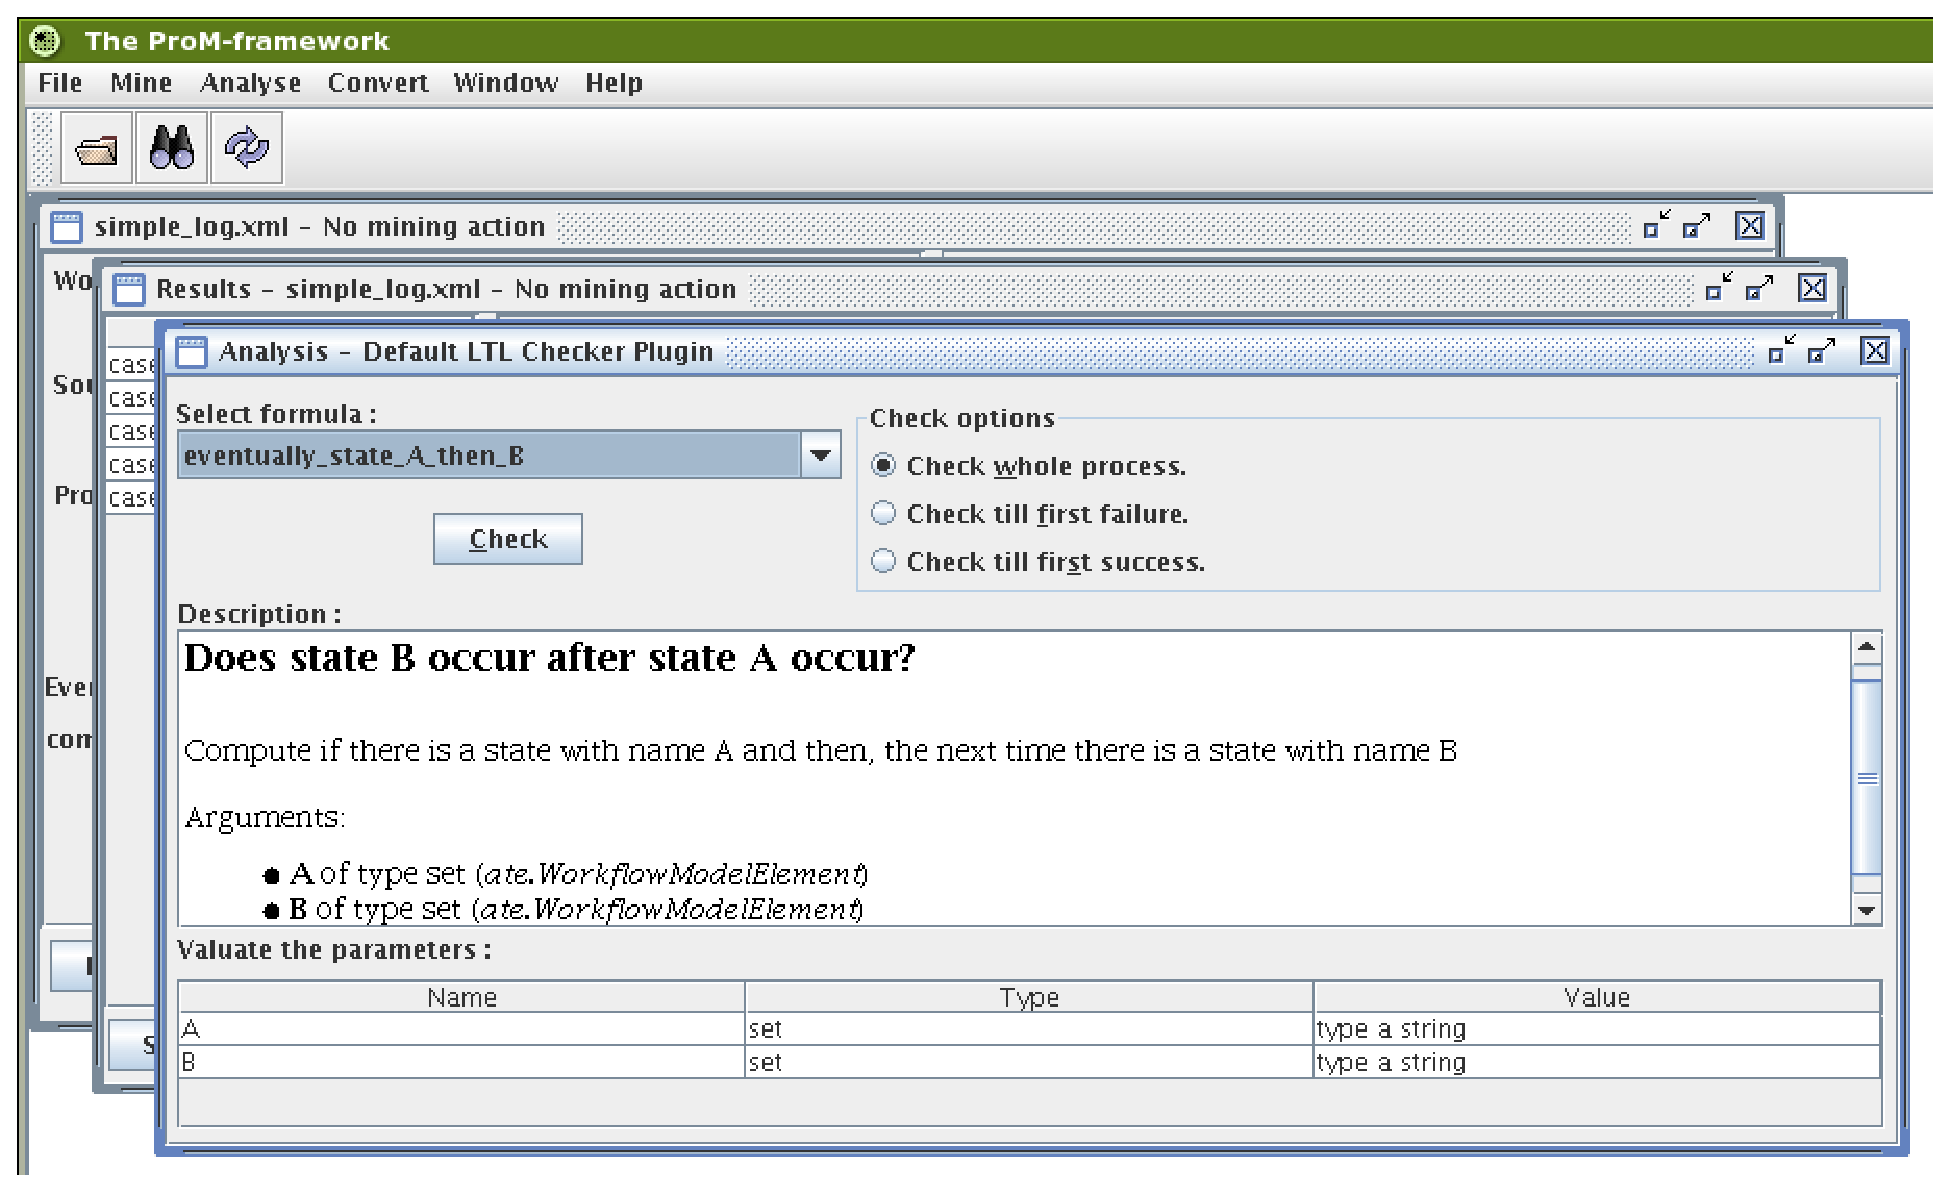
\includegraphics[scale=0.4]{images/ltlchecker-valuate-params-cutted.eps}
    \caption{Fill in some parameters in the Template GUI.}
    \label{plugingui:valuateparameters}
\end{figure}

It is up to you to fill in the values you want for the different parameters.
Every row of the table exists of three columns: a name, a type and a value.
Initially every parameter has an initial value. For \textit{number} attribute parameters
it is \textit{0.0}, for \textit{date} it is the date of today formatted in the format
specified by the definition of the attribute, for both \textit{string} and
\textit{set} attribute parameters the initial value is \textit{type a string}.

You can only fill in those values that are acceptable values for the different
kinds of attribute types. This means that every value, in case its type is
number or date, is parsed to a value of that type. If this parsing is
successful, the new value is placed into the table, if the parsing does not
succeed the old value does not change.

It is good to know that you can only fill in literals. That is, attribute
names, string lists and other formulae are not accepted as values, they are
interpreted as strings and, in cases of date and number attributes, they are
parsed as dates or numbers respectively.

Once you have set the values you want for the parameters, you can use the next
part of the Template GUI to set some check options. This part is right of the
list with formulae. There are three options
you can choose from:
\begin{enumerate}
    \item \textit{Check whole process} Check all process instances in the log
    for the selected formula.
    \item \textit{Check till first failure} Check all process instances in the
    log, but stop at the first encountered process instance \textbf{not
    having} the property specified by the selected formula.
    \item \textit{Check till first success} The reverse of the previous item.
    Check all process instances in the log, but stop at the first encountered
    process instance \textbf{having} the property.
\end{enumerate}

\begin{figure}[H]
    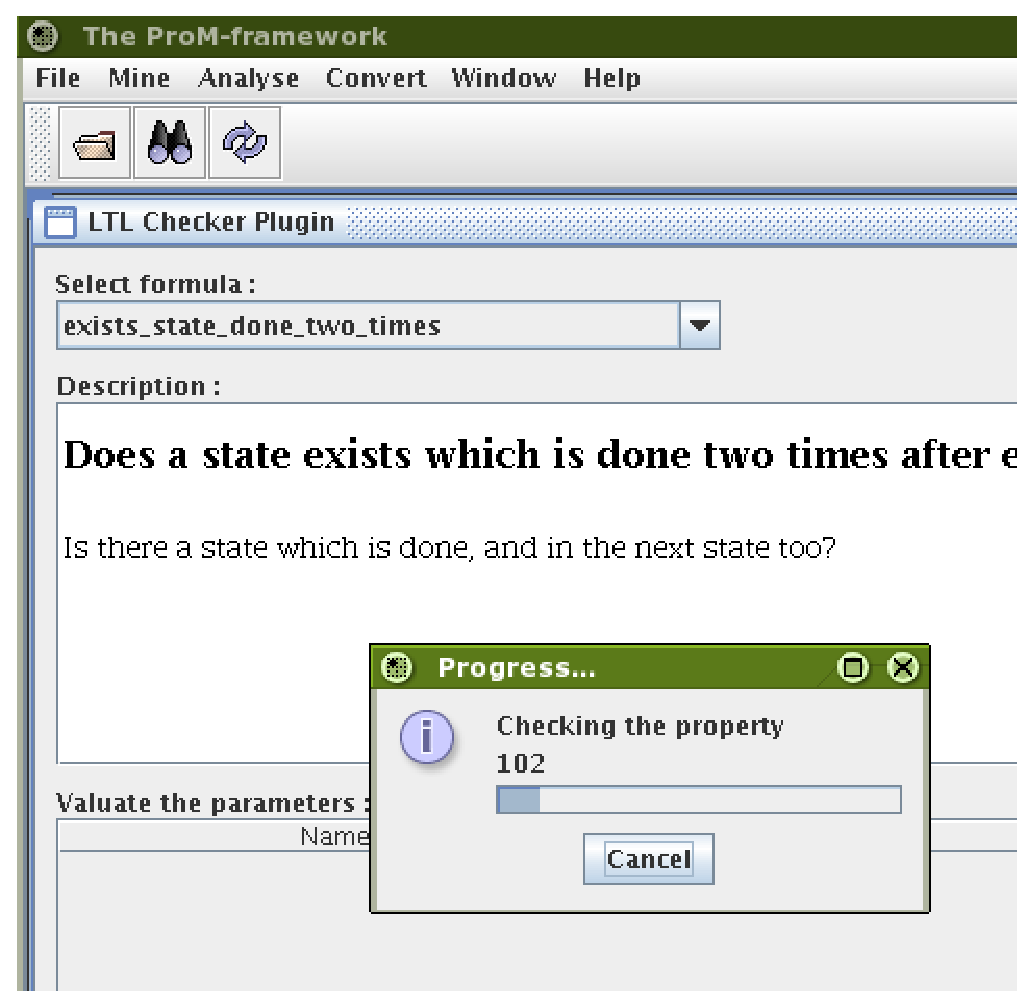
\includegraphics[scale=0.4]{images/ltlchecker-checking-cutted.eps}
    \caption{The actual checking is going.}
    \label{plugingui:checking}
\end{figure}

If you have set the check option you want and the parameters are valuated as you wish,
you can click the \menu{Check} button to start the actual check ( Figure
\ref{plugingui:checking} ). You will find this \menu{Check} button below the list
with formulae, so in case you select a formula without any parameters, you can
then click directly the \menu{Check} button to start checking.

By the first check, the sets for the defined set
attributes are created ( these sets are reused by next checks ) and the check
starts hereafter. While checking, the progress of the check is displayed together with the name of
the 'current' instance ( On the figure, the names are just numbers, but it can
be every string ). If you want to stop the checking, just click the
\menu{Cancel} button on the progress window. After the check is done, a new window is displayed: the
results window.

\section{Viewing the Results}
\label{plugingui:results}
\index{LTL Checker Plugin!Viewing the results of a check}
\index{Results window}

\begin{figure}[H]
    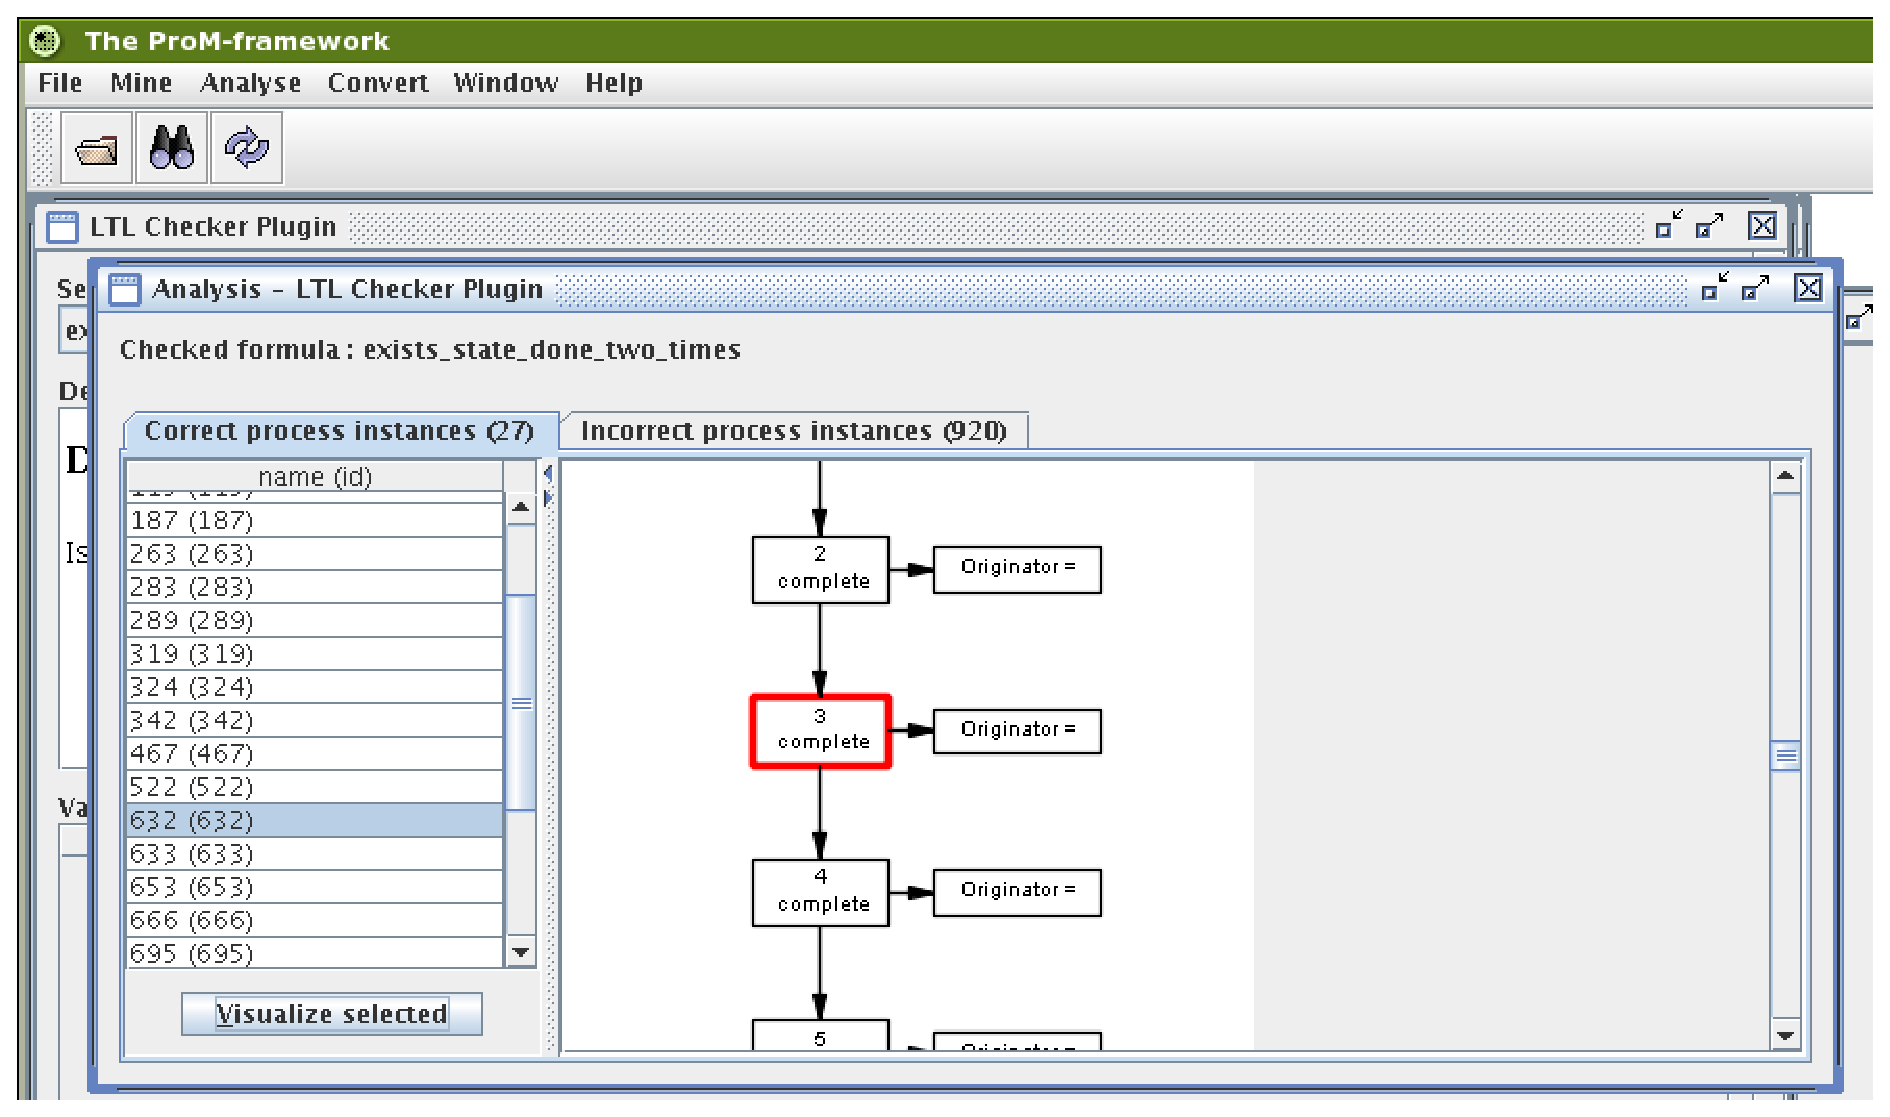
\includegraphics[scale=0.4]{images/ltlchecker-check-results-cutted.eps}
    \caption{The window with the results: a tab with correct instances and one
    with incorrect instances.}
    \label{plugingui:results}
\end{figure}

On the results window you see first the name of the checked formula. Below
this text, the window is divided
into two tabs: one with the correct instances and one with the incorrect
instances. Both tabs have the same structure. In the title of the tab, between
parentheses the number of instances on that tab is given. So you can easily
see how much instances of the log are correct or incorrect ( Figure
\ref{plugingui:results}).

On the tab itself you see two parts: the actual table with the instances on
the left and a visualization pane on the right. In this table, the process
instances are listed, the name of the instances
exists of the process instance name and between parentheses the rank of the
instance in the log. Now you can easily see how the correct and incorrect instances are
distributed over the log.

The visualization pane on the right hand side of the log can be used to
visualize one of the instances listed in the table. Just select an instance and
click the \menu{Visualize selected} button
to create a visualization of the instance. 

Both the lists of correct and
incorrect instances can be exported or reused as ordinary logs can be.
Furthermore, a visualization can be exported too.

\section{Exporting the Results}
\label{plugingui:exproting}
\index{LTL Checker Plugin!Exporting the results}
\index{Exporting in the ProM framework}

\begin{figure}[H]
    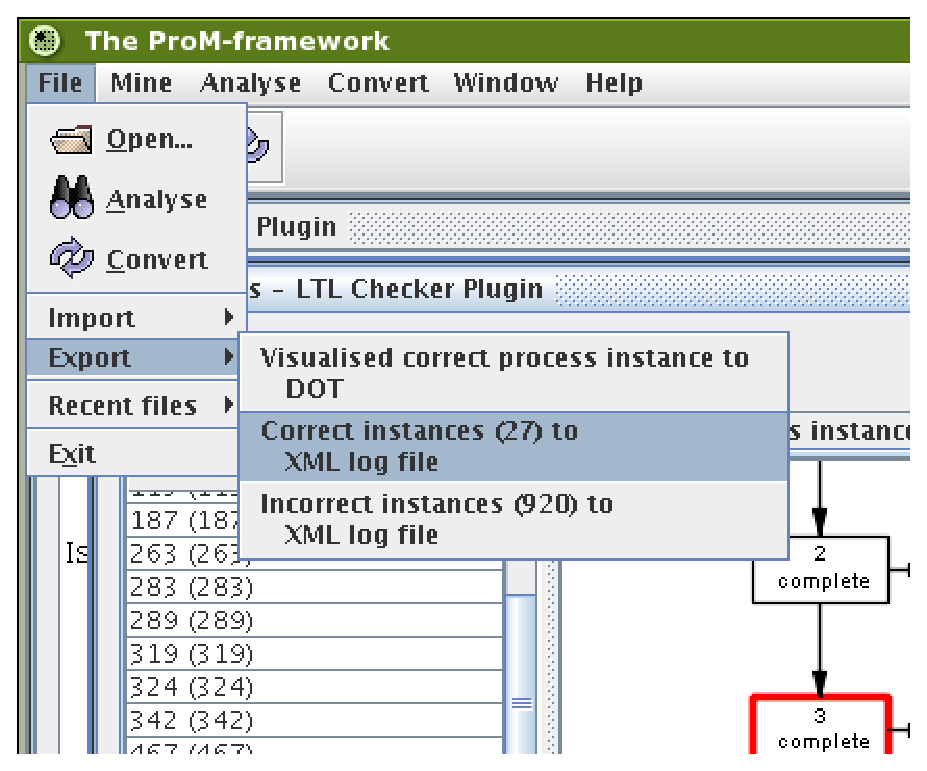
\includegraphics[scale=0.5]{images/framework-results-exportmenu-cutted.eps}
    \caption{Exporting the results: logs and visualizations.}
    \label{plugingui:export}
\end{figure}

Exporting of the results, both the lists with instances and the
visualizations, is very easy. As in Figure \ref{plugingui:export} can be seen,
just go to the \menu{File} menu, sub menu \menu{Export} and click on the desired
export. A save dialog is displayed then, in which you can give a name and a place to save the export to.

\section{Reusing the results}
\label{plugingui:reusing}
\index{LTL Checker Plugin!Reusing the results}

\begin{figure}[H]
    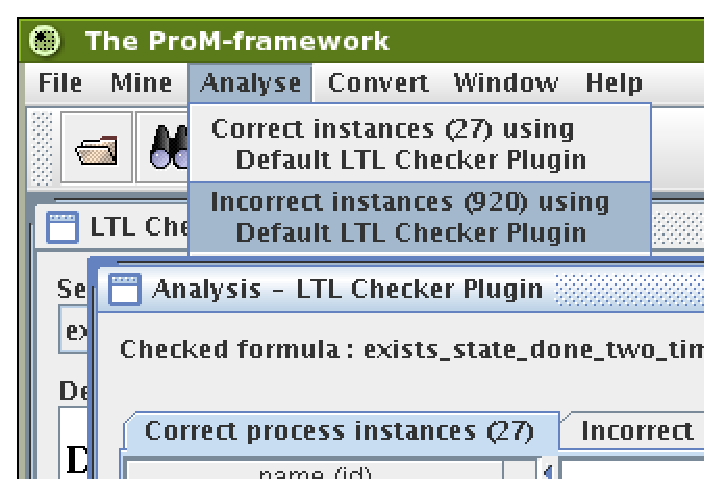
\includegraphics[scale=0.5]{images/framework-results-defaultmenu-cutted.eps}
    \caption{On the results the LTL Checker analysis can be done again with
    the Default LTL Checker plugin.}
    \label{plugingui:defaultagain}
\end{figure}

It is possible to use the results of a check again in the ProM framework, for
example as input to the LTL Checker plugins. Both the Default LTL Checker
plugin ( Figure
\ref{plugingui:defaultagain} ) and the "normal"
LTL Checker Plugin ( Figure \ref{plugingui:genericagain} ) can be applied
on a result log, either the list with the correct instances or the list with
the incorrect instances.

\begin{figure}[H]
    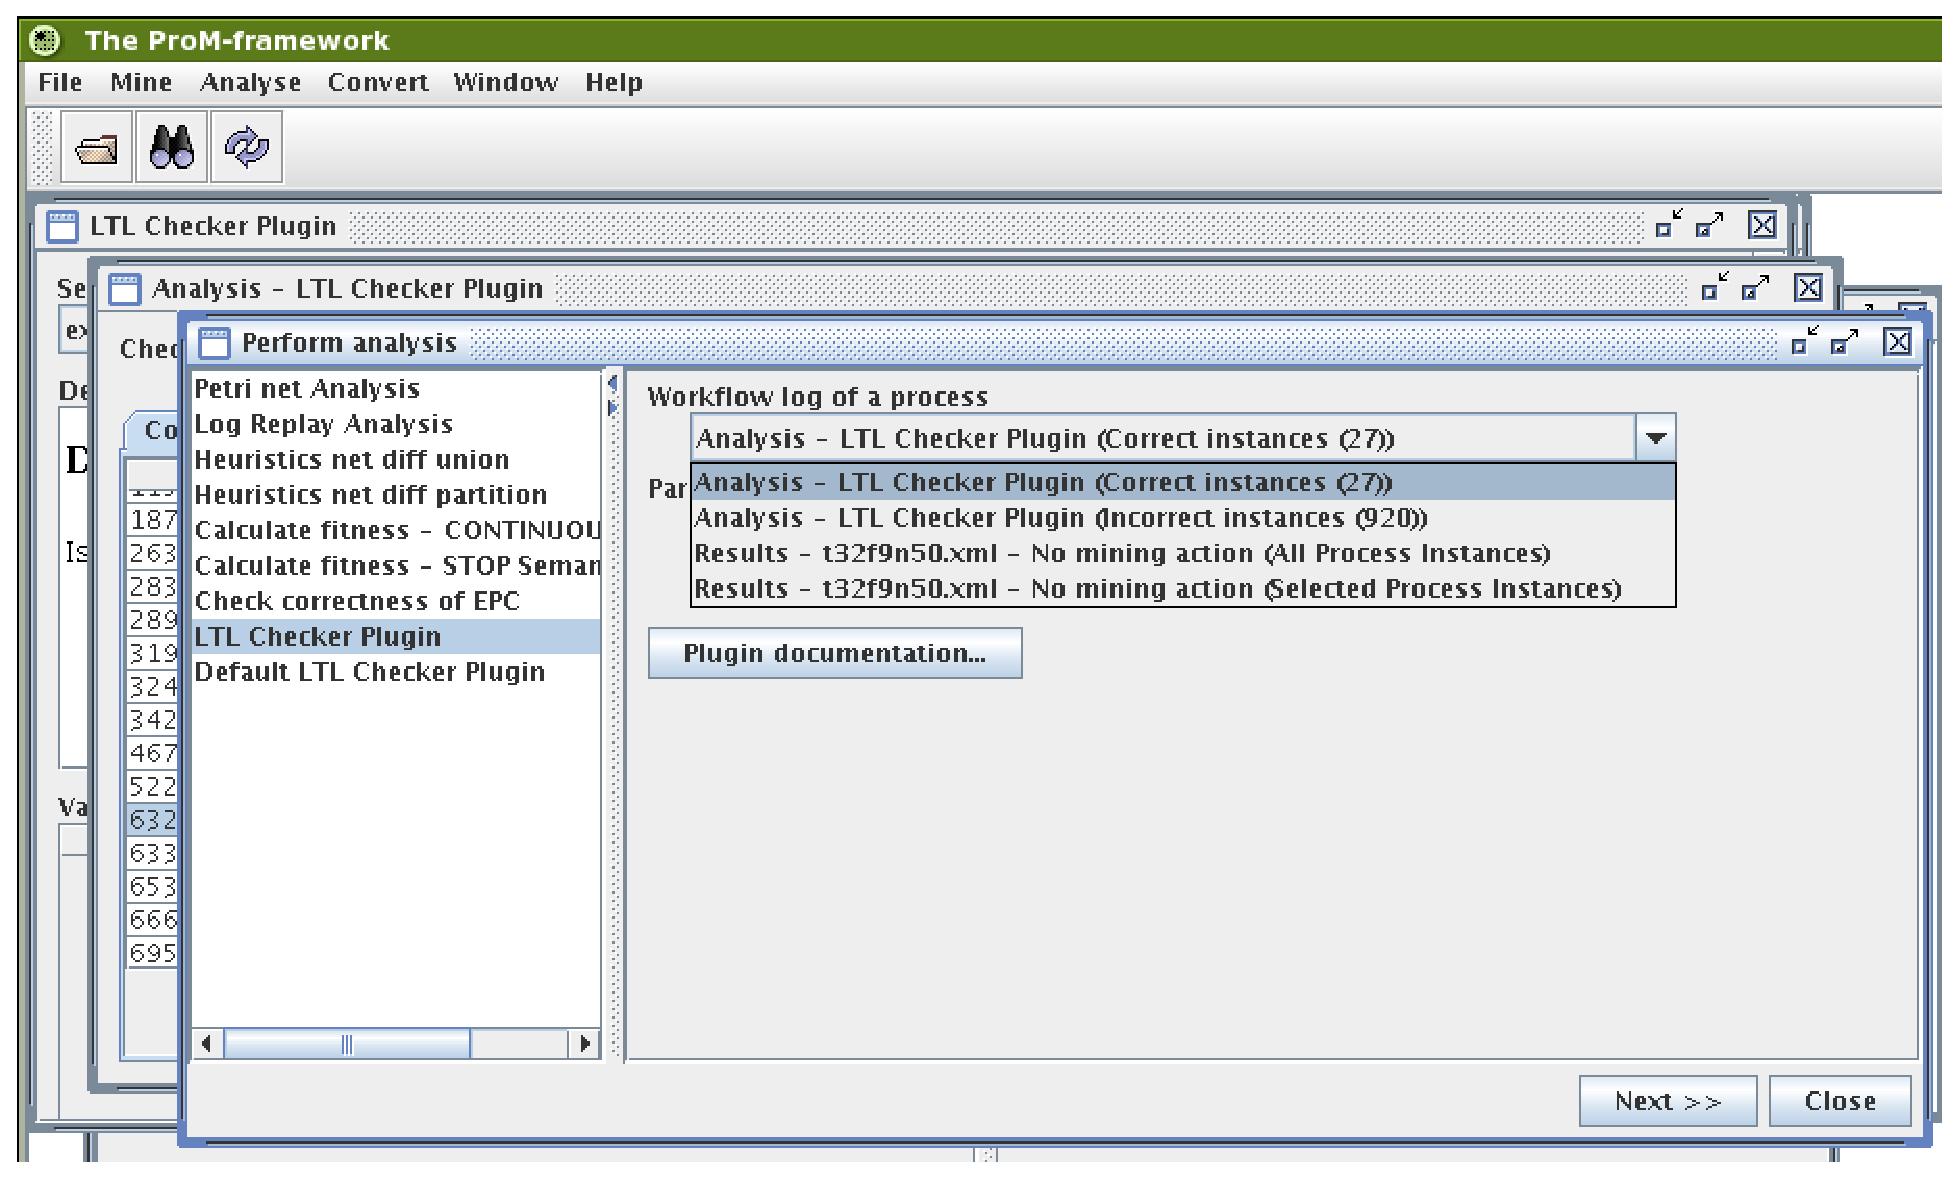
\includegraphics[scale=0.4]{images/framework-log-and-results-and-ltl-analyse-cutted.eps}
    \caption{On the results the LTL Checker analysis can be done again, also
    the using the LTL Checker plugin.}
    \label{plugingui:genericagain}
\end{figure}

So it is possible to refine logs as far as you want, till the point you
are satisfied. For example, you can filter first all instances with property
P, and then on those instances check for property Q. Of course, you can create
a formula R equivalent to P $\wedge$ Q, which gives the same results, but then, you
should know beforehand you want to check both P and Q. Furthermore, how
smaller the log, how faster the check.

\begin{figure}[H]
    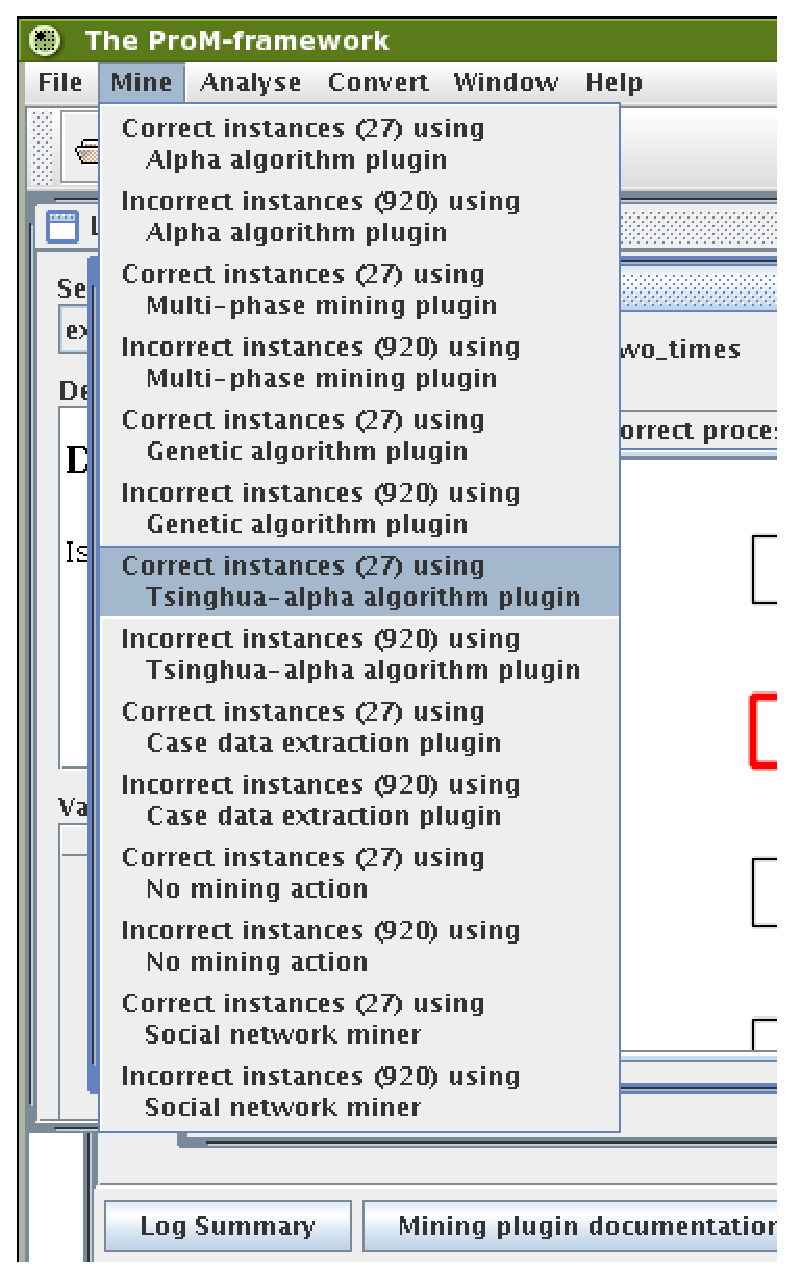
\includegraphics[scale=0.4]{images/framework-log-and-ltl-minemenu-cutted.eps}
    \caption{On the results the LTL Checker you can also run a mining
    algorithm.}
    \label{plugingui:mine}
\end{figure}

Not only the LTL Checker plugins can be used on the result logs, other plugins
can be used too. For example the mining algorithms. In Figure
\ref{plugingui:mine} you see the \menu{Mine} menu containing all the possible
combinations of result log and mining algorithm, just choose the desired item
to start the mining.
